% Options for packages loaded elsewhere
\PassOptionsToPackage{unicode}{hyperref}
\PassOptionsToPackage{hyphens}{url}
%
\documentclass[
  english,
  man]{apa6}
\usepackage{lmodern}
\usepackage{amssymb,amsmath}
\usepackage{ifxetex,ifluatex}
\ifnum 0\ifxetex 1\fi\ifluatex 1\fi=0 % if pdftex
  \usepackage[T1]{fontenc}
  \usepackage[utf8]{inputenc}
  \usepackage{textcomp} % provide euro and other symbols
\else % if luatex or xetex
  \usepackage{unicode-math}
  \defaultfontfeatures{Scale=MatchLowercase}
  \defaultfontfeatures[\rmfamily]{Ligatures=TeX,Scale=1}
\fi
% Use upquote if available, for straight quotes in verbatim environments
\IfFileExists{upquote.sty}{\usepackage{upquote}}{}
\IfFileExists{microtype.sty}{% use microtype if available
  \usepackage[]{microtype}
  \UseMicrotypeSet[protrusion]{basicmath} % disable protrusion for tt fonts
}{}
\makeatletter
\@ifundefined{KOMAClassName}{% if non-KOMA class
  \IfFileExists{parskip.sty}{%
    \usepackage{parskip}
  }{% else
    \setlength{\parindent}{0pt}
    \setlength{\parskip}{6pt plus 2pt minus 1pt}}
}{% if KOMA class
  \KOMAoptions{parskip=half}}
\makeatother
\usepackage{xcolor}
\IfFileExists{xurl.sty}{\usepackage{xurl}}{} % add URL line breaks if available
\IfFileExists{bookmark.sty}{\usepackage{bookmark}}{\usepackage{hyperref}}
\hypersetup{
  pdftitle={Mapping factors associated with adolescents' emotion dysregulation: A text-mining based systematic review},
  pdfkeywords={keywords},
  hidelinks,
  pdfcreator={LaTeX via pandoc}}
\urlstyle{same} % disable monospaced font for URLs
\usepackage{graphicx,grffile}
\makeatletter
\def\maxwidth{\ifdim\Gin@nat@width>\linewidth\linewidth\else\Gin@nat@width\fi}
\def\maxheight{\ifdim\Gin@nat@height>\textheight\textheight\else\Gin@nat@height\fi}
\makeatother
% Scale images if necessary, so that they will not overflow the page
% margins by default, and it is still possible to overwrite the defaults
% using explicit options in \includegraphics[width, height, ...]{}
\setkeys{Gin}{width=\maxwidth,height=\maxheight,keepaspectratio}
% Set default figure placement to htbp
\makeatletter
\def\fps@figure{htbp}
\makeatother
\setlength{\emergencystretch}{3em} % prevent overfull lines
\providecommand{\tightlist}{%
  \setlength{\itemsep}{0pt}\setlength{\parskip}{0pt}}
\setcounter{secnumdepth}{-\maxdimen} % remove section numbering
% Make \paragraph and \subparagraph free-standing
\ifx\paragraph\undefined\else
  \let\oldparagraph\paragraph
  \renewcommand{\paragraph}[1]{\oldparagraph{#1}\mbox{}}
\fi
\ifx\subparagraph\undefined\else
  \let\oldsubparagraph\subparagraph
  \renewcommand{\subparagraph}[1]{\oldsubparagraph{#1}\mbox{}}
\fi
% Manuscript styling
\usepackage{upgreek}
\captionsetup{font=singlespacing,justification=justified}

% Table formatting
\usepackage{longtable}
\usepackage{lscape}
% \usepackage[counterclockwise]{rotating}   % Landscape page setup for large tables
\usepackage{multirow}		% Table styling
\usepackage{tabularx}		% Control Column width
\usepackage[flushleft]{threeparttable}	% Allows for three part tables with a specified notes section
\usepackage{threeparttablex}            % Lets threeparttable work with longtable

% Create new environments so endfloat can handle them
% \newenvironment{ltable}
%   {\begin{landscape}\begin{center}\begin{threeparttable}}
%   {\end{threeparttable}\end{center}\end{landscape}}
\newenvironment{lltable}{\begin{landscape}\begin{center}\begin{ThreePartTable}}{\end{ThreePartTable}\end{center}\end{landscape}}

% Enables adjusting longtable caption width to table width
% Solution found at http://golatex.de/longtable-mit-caption-so-breit-wie-die-tabelle-t15767.html
\makeatletter
\newcommand\LastLTentrywidth{1em}
\newlength\longtablewidth
\setlength{\longtablewidth}{1in}
\newcommand{\getlongtablewidth}{\begingroup \ifcsname LT@\roman{LT@tables}\endcsname \global\longtablewidth=0pt \renewcommand{\LT@entry}[2]{\global\advance\longtablewidth by ##2\relax\gdef\LastLTentrywidth{##2}}\@nameuse{LT@\roman{LT@tables}} \fi \endgroup}

% \setlength{\parindent}{0.5in}
% \setlength{\parskip}{0pt plus 0pt minus 0pt}

% \usepackage{etoolbox}
\makeatletter
\patchcmd{\HyOrg@maketitle}
  {\section{\normalfont\normalsize\abstractname}}
  {\section*{\normalfont\normalsize\abstractname}}
  {}{\typeout{Failed to patch abstract.}}
\makeatother
\shorttitle{ADOLESCENT EMOTION DYSREGULATION}
\author{Caspar J. van Lissa\textsuperscript{1,2}}
\affiliation{
\vspace{0.5cm}
\textsuperscript{1} Utrecht University faculty of Social and Behavioral Sciences, department of Methodology \& Statistics\\\textsuperscript{2} Open Science Community Utrecht}
\authornote{Caspar van Lissa, Department of Methodology and Statistics, Utrecht
University, P.O. Box 80140, 3508 TC, Utrecht, The Netherlands. E-mail:
C.vanLissa@uu.nl. This work is supported by a NWO Veni grant (NWO
grant number VI.Veni.191G.090).


Correspondence concerning this article should be addressed to Caspar J. van Lissa, Padualaan 14, 3584CH Utrecht, The Netherlands. E-mail: c.j.vanlissa@uu.nl}
\keywords{keywords\newline\indent Word count: X}
\DeclareDelayedFloatFlavor{ThreePartTable}{table}
\DeclareDelayedFloatFlavor{lltable}{table}
\DeclareDelayedFloatFlavor*{longtable}{table}
\makeatletter
\renewcommand{\efloat@iwrite}[1]{\immediate\expandafter\protected@write\csname efloat@post#1\endcsname{}}
\makeatother
\usepackage{lineno}

\linenumbers
\usepackage{csquotes}
\ifxetex
  % Load polyglossia as late as possible: uses bidi with RTL langages (e.g. Hebrew, Arabic)
  \usepackage{polyglossia}
  \setmainlanguage[]{english}
\else
  \usepackage[shorthands=off,main=english]{babel}
\fi

\title{Mapping factors associated with adolescents' emotion dysregulation: A text-mining based systematic review}

\date{}

\abstract{
Test me
}

\begin{document}
\maketitle

A key developmental challenge in adolescence is acquiring mature emotion
regulation skills (Crone \& Dahl, 2012; Zimmermann \& Iwanski, 2014). Emotion regulation is integral to
mental health(Aldao, Nolen-Hoeksema, \& Schweizer, 2010; Braet et al., 2014; Schäfer, Naumann, Holmes, Tuschen-Caffier, \& Samson, 2017)
and social functioning (Reindl, Gniewosz, \& Reinders, 2016). For as many
as one in five people, adolescence marks the onset of emotion
regulation-related mental illness, which can persist throughout the life course
(see Lee et al., 2014). It is therefore crucial to identify which
risk factors and environmental hazards render some adolescents more susceptible
to emotional difficulties than others. Although there is an abundance of
empirical work on adolescents' emotion regulation, the literature is somewhat
fragmented, as the topic has been investigated from different (sub)disciplines.
This study seeks to overcome this limitation by mapping all factors currently
thought to be relevant to adolescent emotion regulation, based on a systematic
review and bibliographic analysis.

\hypertarget{why-adolescence-is-an-important-life-phase-for-emotion-regulation}{%
\subsection{Why adolescence is an important life phase for emotion regulation}\label{why-adolescence-is-an-important-life-phase-for-emotion-regulation}}

Adolescence is defined as a life phase ranging from pubertal onset to
adult-like independence (Steinberg, 2014). This definition
invokes both biological- and socio-cultural factors. It has been argued that,
due to accellerated pubertal onset and delayed transitions to adult roles,
adolescence now ranges from 10-24 years in the modern Western world
(Sawyer, Azzopardi, Wickremarathne, \& Patton, 2018).

Adolescence is increasingly seen as a developmentally sensitive period for
mature emotion regulation skills. During this period, children experience rapid
biological, cognitive, and social changes that prompt new emotional
experiences, and tax existing regulatory abilities
(Steinberg, 2014). At the same time, the staggered
development of motivational-emotional and regulatory brain circuits gives rise
to a maturity gap, where youngsters pursue new experiences in life and love,
without being fully prepared to cope with the emotional outcomes
(Crone \& Dahl, 2012). Due to these coalescing changes,
adolescents display a restricted repertoire of emotion regulation strategies
compared to younger or older individuals
(Zimmermann \& Iwanski, 2014). Consequently, adolescents experience
more frequent and intense (negative) emotions than children or adults (see Silk, Steinberg, \& Morris, 2003). The literature thus paints a picture of
adolescence as a chrysalis for emotional development: Children enter this stage
with emotion regulation skills adapted to the challenges of childhood. During
adolescence, emotional systems are rearranged substantially. These changes
render adolescents temporarily vulnerable to emotional dysregulation, but
ultimately serve a functional role in acquiring mature emotion regulation
skills. Eventually, most adolescents emerge ready to take on the challenges of
early adulthood. Unfortunately, a sizeable proportion of adolescents instead
manifests enduring emotional difficulties.

\hypertarget{the-consequences-of-difficulties-in-emotion-regulation}{%
\subsection{The consequences of difficulties in emotion regulation}\label{the-consequences-of-difficulties-in-emotion-regulation}}

The
consequences of difficulties in emotion regulation are extensive,
well-documented, and persist throughout the life course. Meta-analyses indicate
that such difficulties are associated with externalizing, and more strongly,
with internalizing psychopathology
(Aldao et al., 2010; Schäfer et al., 2017). Individuals who engage in maladaptive
emotion regulation strategies also experience more negative emotions,
diminished well-being, and greater strain in interpersonal relationships
(Bell \& Calkins, 2000; Gross \& John, 2003).
Given the
prevalence of emotional difficulties and their extensive implications for
individual mental health, wellbeing, and social functioning, and downstream
cost to society as a whole (Lee et al., 2014), it is essential to
have a solid understanding of the risk factors associated with adolescents'
emotion regulation difficulties.

\hypertarget{existing-relevant-theory}{%
\subsection{Existing relevant theory}\label{existing-relevant-theory}}

Theory is of paramount importance when seeking to understand or explain a
phenomenon. Although there are many relevant theories, none have specifically
addressed emotion regulation development in adolescence. Several recent
publications have undertaken the monumental task of comprehensively reviewing
theory relevant to emotional development
(Buss, Cole, \& Zhou, 2019; Riediger \& Klipker, 2014). Thanks, in part, to their efforts,
we can provide a summary review of the theoretical landscape as context for our
empirical contribution.
Two theories widely invoked to frame research on development, including
emotional development, are Bronfenbrenner's bioecological model, and Sameroff's
transactional model. Bronfenbrenner's model
(Bronfenbrenner \& Morris, 2007) describes how the environment
shapes individual development. Each individual is imbued with certain
biological predispositions, and develops over time, in interaction with
contextual influences. These influences range from the microsystem, composed of
those people close to the individual, to the macrosystem, consisting of
indirect political and economic influences, to the exosystem, consisting of
cultural norms and values. Sameroff's model is somewhat compatible with the
bioecological model ({\textbf{???}}), but focuses more
on the interplay between nature and nurture. It conceptualizes development as a
product of reciprocal influences between the child and the environment.
Sameroff distinguishes between proximal influences, for instance, through
parents (the microsystem in Bronfenbrenner's model), and distal influences;
structural factors indirectly shaping development, like socio-economic status,
schools, and the community (macro- and exosystem). With increasing age, distal
influences gradually gain ground on proximal influences.

Turning now towards theories specifically addressing emotion regulation in
adolescence, Hall's notion of \enquote{storm and stress} is one of the oldest (see Arnett, 1999). It describes how hormonal changes diminish
self-control and increase reactivity, leading to difficulties in emotion
regulation, conflict with parents, and risky behavior. Recent work provides a
more nuanced perspective on this theory. For example, although the notion of
diminished self-control and increased emotional reactivity has been upheld, it
has been recast as a necessary change that facilitates emotional maturation
(Crone \& Dahl, 2012), at the risk of emotional
disturbance (Arnett, 1999; Lee et al., 2014).
More recently, Sroufe (1995) presented
a theory focused on normative emotional development in early childhood. It
argues that, as children grow older, their increasing self-regulatory abilities
drive a transition from external emotion regulation by primary caregivers
towards autonomous emotion regulation. This theory focuses on two drivers of
development: social and cognitive influences. Social influences mainly occur
through parents' co-regulation, parenting behaviors, and parent-child
attachment. Cognitive influences occur through the development of the central
nervous system (CNS), cognition, and self-regulation. Several other theories,
introduced below, have extemporized on these sources of influence.

The emphasis on neorocognitive development as a driver of emotional
development, including emotion regulation development, is echoed in several
other models. For example, polyvagal theory closely links emotional experience
- and regulation - to autonomous nervous system functioning
(Porges, 1995). A more recent neorocognitive theory, with
substantial relevance to adolescents' emotion regulation development, is Crone
and Dahl's model of social-affective engagement and goal flexibility
(Crone \& Dahl, 2012). This theory is based on the notion
of a \enquote{maturity gap} in middle-adolescence, arising from a developmental
asymmetry between motivational and inhibitory brain circuits
({\textbf{???}}; Cracco, Goossens, \& Braet, 2017). However, it sets out to explain - to
a greater extent than other writings - adolescents' diverging destinies; the
question why some youngsters flourish while others languish. Crone and Dahl
argue that adolescents' cognitive engagement is dynamically responsive to
social and motivational goal salience. This flexibility, on the one hand,
prepares adolescents to effectively engage cognitive systems in novel
challenging situations in a way that facilitates developing mature regulatory
abilities. On the other hand, it places them at risk to act impulsively in
pursuit of peer approval. This theory focuses primarily on cognitive factors
and the role of peers, with less attention to factors such as parenting.

A theory focused specifically on parents' role in emotion regulation
development is Morris' tripartite model (2007). It
describes three pathways through which parents shape emotion regulation
development: Through observation and modeling, parenting practices, and the
emotional family climate, which in turn involves attachment and marital
relationship quality. Morris and colleagues also emphasize the relevance of
fathers and siblings, and others have adapted the tripartite model to describe
the role of peers in adolescents' emotion regulation development
(Reindl et al., 2016).

Aside from theories of emotional development, theories of the phenomenon of
emotion regulation are also somewhat relevant. One influential theory is Gross'
(2013) process model, which describes the
process of emotion regulation, from eliciting cue to ultimate response.
Individuals modulate the different stages of this process using strategies,
consciously or otherwise. The effectiveness, desireability, and consequences of
different strategies depend on the cultural context (see Bariola, Gullone, \& Hughes, 2011). Similar to Gross' theory, the social
information processing theory of emotion also describe the role of intrapsychic
processes and strategies in emotion experience and reulation
(Lemerise \& Arsenio, 2000).

Another theory worth mentioning in this context is
Holodynski and Friedlmeier (2006)'s internalization model of emotional
development. It applies Vygotsky's theory of development to the domain of
emotion, and presents a detailed integrated model of emotional experience and
regulation. Like Sroufe's work, this work describes a transition from
interpersonal to intrapersonal emotion regulation. Other important features of
this work include the interplay between emotion and communication, and the
internalization of the socio-cultural symbolic function of emotion throughout
development.

\hypertarget{shortcomings-of-the-theory}{%
\subsection{Shortcomings of the theory}\label{shortcomings-of-the-theory}}

Existing theoretical models have several limitations. One crucial shortcoming
is the lack of explicit attention to the life phase of adolescence. This is
unfortunate, as empirical research consistently indicates that adolescence is a
crucial life phase for emotion regulation development. Adolescence differs
qualitatively from infancy, childhood, and adulthood. It is therefore
insufficient to simply extrapolate theories focused on these ages. Other
theories do focus on adolescence specifically (e.g., Crone \& Dahl, 2012), but only address emotion regulation
in passing. A second, related, shortcoming is that some relevant theories lack
a developmental component (see Buss et al., 2019; Crone \& Dahl, 2012). A third shortcoming is that theories
vary widely in scope: Some are very broad and all-encompassing, but somewhat
non-specific, such as the biopsychosocial models of Bronfenbrenner and
Sameroff. Others describe a specific phenomenon in great detail, but are not
embedded in a larger unifying framework. Examples include Morris' tripartite
model, Crone and Dahl's model, and polyvagal theory. It would be beneficial to
bridge these two levels of theory. One limitation echoed across many
publications in this field is that more theory formation is required to provide
a unified framework that could guide future empirical work. The present study
seeks to aid such theory development, by providing an inductive conceptual
review of the field.

\hypertarget{bottom-up-insights-from-narrative-reviews}{%
\subsection{Bottom-up insights from narrative reviews}\label{bottom-up-insights-from-narrative-reviews}}

While theory provides a top-down understanding of an area of research,
literature reviews can provide a bottom-up, inductive understanding. Given the
noted absence of a single overarching theory, reviews might provide additional
insight into factors considered relevant in the etiology of adolescents'
emotion regulation competencies. For example, a review by
Bariola et al. (2011) addresses individual psychological factors
such as temperament, and biological factors like neurocognitive development and
genetic predispositions. Furthermore, they address proximal social influences,
including parents, teachers, and peers, and specific mechanisms through which
these individuals exert their influence, including parenting and modeling.
Finally, they address distal factors, including the role of culture and the
media. Barriola and colleagues also offer recommendations for future research,
calling for research on the role of parents beyond early
childhood, and including the role of fathers - a limitation which has since
been addressed by a new wave of empirical research on fathers' role in
emotional development (Van Lissa \& Keizer, 2020; Van Lissa, Keizer, Van Lier, Meeus, \& Branje, 2019).

Another review, by Coe-Odess, Narr, and Allen (2019), offers a nuanced
discussion of several issues that complement prior publications in this field.
For instance, the authors cover the implications of physiological changes in
detail, including neurocognitive development and pubertal maturation. As
adolescents become increasingly individuated, conflict with parents peaks. This
conflict, in turn, impacts emotion regulation, both in terms of day-to-day mood
variability and dispositional emotion dysregulation (see also Van Lissa, Hawk, Koot, Branje, \& Meeus, 2017). As parental importance diminishes,
adolescents become increasingly oriented towards peers. This includes increased
sensitivity to social status and norms, along with the associated increase in
peer pressure and risk taking. Pubertal development also initiates the
emergence of sexual and romantic behavior, and the intensification of both
biological sex differences and gender stereotyped behavior. With regard to the
process of emotion regulation, Coe-Odess and colleagues discuss the importance
of strategies, and point out that, in addition to negative emotionality,
positive emotionality also peaks in adolescence. Relatedly, the authors
describe how hormonal changes precipitate an increased stress response, which
might help explain adolescents' greater susceptibility to emotion
dysregulation. Finally, going beyond the implications of cognitive development
discussed in other publications, the authors discuss how an greater capacity
for abstract thought relates to identity formation - a key challenge in
adolescence ({\textbf{???}}) - and to increased emotional
understanding, and by extension, empathy (see also Van Lissa et al., 2014).

There are notable parallels between the relevant factors highlighted by these
narrative reviews, and the aforementioned theoretical literature. Nevertheless,
these literature reviews also touch upon issues that have received little
attention in theoretical work. This highlights the value of both top-down and
bottom-up approaches to understanding the phenomenon of adolescents' emotion
regulation. One remaining limitation is that, to date, all reviews in this
field have been unstructured narrative reviews. The present publication seeks
to further complement preceding work by conducting a comprehensive empirical
literature review, and mapping the factors associated with adolescent emotion
regulation.

\hypertarget{the-present-paper}{%
\subsection{The present paper}\label{the-present-paper}}

The present paper aims to develop a nomological network of the constructs
related to adolescent emotion dysregulation, based on a systematic review of
the literature. A nomological network is a diagrammatic representation of a
phenomenon; a proto-theoretical device that describes relationships between
constructs relevant to the theory (see Alavi, Archibald, McMaster, Lopez, \& Cleary, 2018). It is a precursor to a more
explicit theory of the phenomenon. The present paper uses an inductive approach
to develop this nomological network. First, we conduct a systematic search to
elicit a corpus of relevant literature. Second, we use text mining techniques
to extract relevant constructs from the corpus. Third, we use a dictionary to
pare down the extracted constructs to meaningful superordinate categories.
Fourth, we map interrelations between these constructs. Fifth, we classify
contstructs as potential predictors or outcomes, and we categorize predictors
by level of analysis.

\hypertarget{methods}{%
\section{Methods}\label{methods}}

\hypertarget{search-strategy}{%
\subsection{Search strategy}\label{search-strategy}}

All searches were conducted on Web of Science. The search strategy was based on
procedures described by Staaks (Staaks, n.d.). First, we
manually constructed a reference set of 15 articles. Then we constructed a
search string to retrieve these articles from Web of Science. The search was
overly inclusive, returning 29 records. As these were all highly relevant, we
updated the reference set to include all 29 results. Next, we tested our search
string, which consisted of synonyms of emotion regulation and adolescence:

\begin{verbatim}
TS=("emotio* regulation" OR "anger regulation" OR "sadness regulation" OR
"emotion* competence" OR "emotion* adjustment" OR "emotio* dysregulation" OR
"anger dysregulation" OR "sadness dysregulation" OR "emotio* problem*" OR
"emotion* maladjustment") AND TS=(adolescent* OR teen* OR pubert* OR youth)
\end{verbatim}

This string returned 6653 results, and matched 25 of the 29 records in the
reference set. Three search terms could be added to match all 29 reference set
items. The terms \texttt{"emotio*\ socialization"\ OR\ "emotio*\ processes"}, as synonyms
of emotion regulation, added 191 new hits. However, many of these hits were not
directly relevant to emotion regulation. The term \texttt{"development*"}, as synonym
of adolescence, added 3628 new hits, many of which were not focused on the age
range of adolescence. We thus deemed these terms to be overly inclusive, and
proceeded with the original search string above.

\hypertarget{deduplication}{%
\subsection{Deduplication}\label{deduplication}}

Duplicates were identified based on exact DOI matches (2
duplicates), and title similarity (54 duplicates).
Manual screening in Rayyan resulted in the removal of an additional 13 duplicates.

\hypertarget{screening}{%
\subsection{Screening}\label{screening}}

Papers were screened based on two main criteria: First, papers had to address emotion regulation, emotional problems, or similar. Second, the target population must overlap (at least in part) with adolescence, defined as the age range from 10-25. Thus, for example, an article reviewing the role of hormonal changes in emotional adjustment throughout the entire life course, including adolescence, would be deemed relevant. Screening was initially conducted in Rayyan QRCI ({\textbf{???}}). Papers were sorted using Rayyan's ranking algorithm. To train the algorithm on exclusion criteria, screening focused on abstracts most likely to be excluded. After coding 559 papers, screening continued in ASReview - a free, open source alternative to Rayyan QRCI ({\textbf{???}}). This program uses text mining and active learning to build a customizable machine learning model for article inclusion. We used a naive Bayes model, and focused on exclusion of irrelevant papers. In ASReview, an additional 541 papers were screened. Screening again focused on articles most likely to be excluded, and continued until, among the most recently screened 100 papers, only 6 were excluded. The screening procedure is detailed in Figure \ref{prismachart}. In total, 6305 papers were retained for analysis.

\begin{figure}
\centering
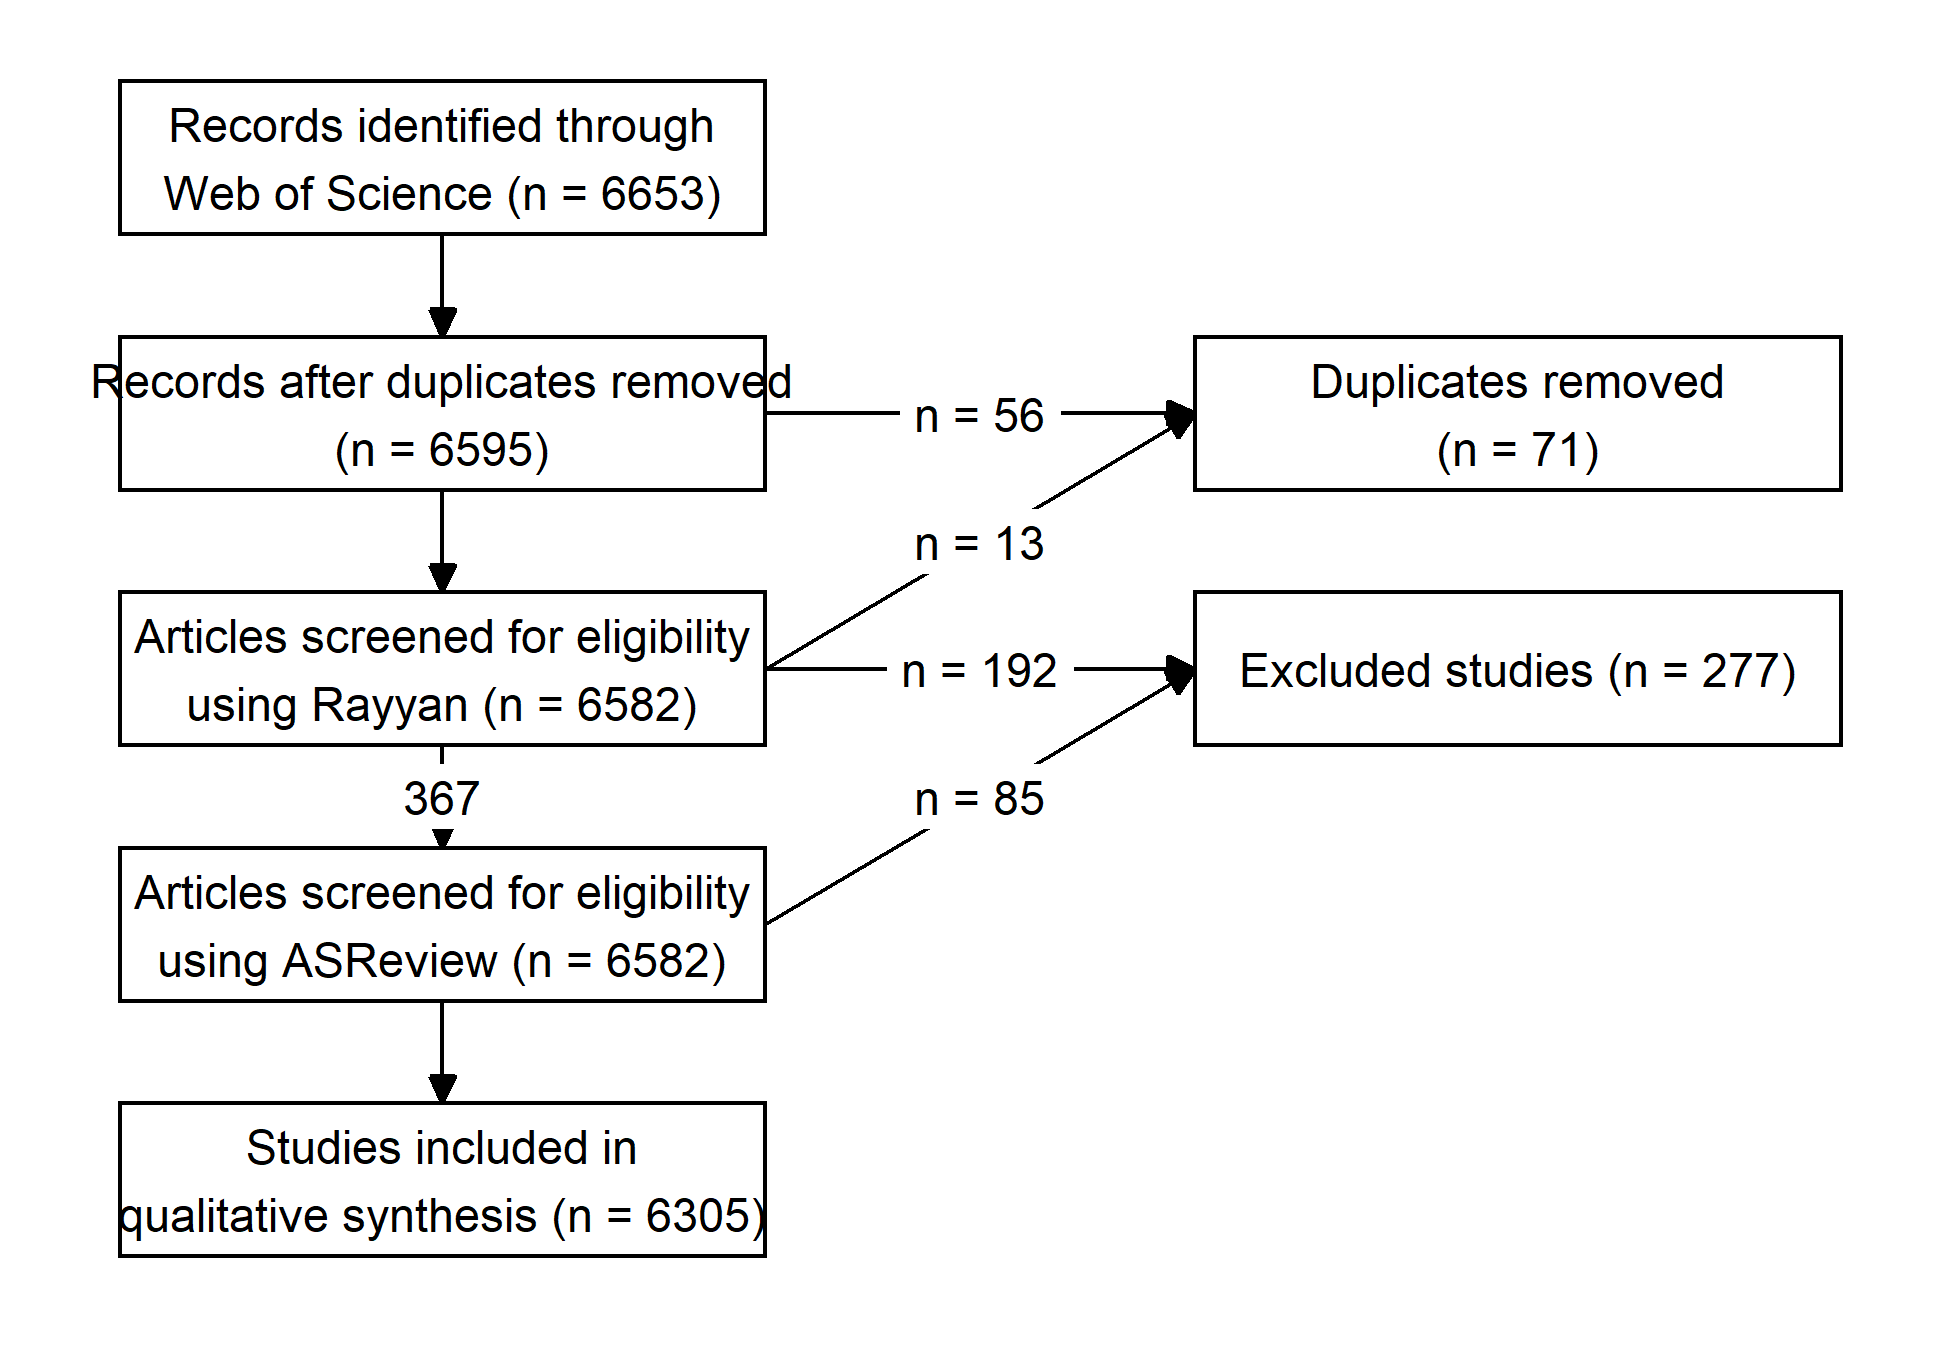
\includegraphics{manuscript_files/figure-latex/prismachart-1.pdf}
\caption{\label{fig:prismachart}Record screening flowchart}
\end{figure}

\hypertarget{analysis-1-keyword-mapping}{%
\section{Analysis 1: Keyword mapping}\label{analysis-1-keyword-mapping}}

For this first analysis, we relied on author-provided keywords.
We extracted keywords by document, and used a dictionary approach
to classify closely related terms.

\hypertarget{analysis-2-abstract-text-mining}{%
\section{Analysis 2: Abstract text mining}\label{analysis-2-abstract-text-mining}}

This second analysis focused on the abstracts of our corpus. Keywords are
carefully chosen to capture the core tenets of a study. However, as authors are
typically limited to 5 keywords, some of a study's nuance may be lost.
Abstracts offer greater freedom of expression, which is a challenge when it
comes to extracting relevant information. We took a two-pronged approach to
extract relevant topic terms from the abstracts. First, we used the natural
language processing technique part-of-speech tagging (POS-tagging) to identify
nouns in the abstract. Using nouns only in text mining can lead to more
interpretable models (Martin \& Johnson, 2015). Secondly, we used
stemming to reduce these nouns to their root form. Finally, we applied a
dictionary approach as before.

offer an incomplete understanding of a study topic due to the limite
authors are typically limited to provide a maximum of
abstracts offer a little more

used part-of-speech tagging, a natural language processing technique

to identify nouns in the abstracts.
, we relied on author-provided keywords. We extracted keywords by document, and used a dictionary approach to classify closely related terms.

\hypertarget{discussion}{%
\section{Discussion}\label{discussion}}

\newpage

\hypertarget{references}{%
\section{References}\label{references}}

\begingroup
\setlength{\parindent}{-0.5in}
\setlength{\leftskip}{0.5in}

\hypertarget{refs}{}
\leavevmode\hypertarget{ref-alaviAligningTheoryMethodology2018}{}%
Alavi, M., Archibald, M., McMaster, R., Lopez, V., \& Cleary, M. (2018). Aligning theory and methodology in mixed methods research: Before Design Theoretical Placement. \emph{International Journal of Social Research Methodology}, \emph{21}(5), 527--540. \url{https://doi.org/10.1080/13645579.2018.1435016}

\leavevmode\hypertarget{ref-aldaoEmotionregulationStrategiesPsychopathology2010}{}%
Aldao, A., Nolen-Hoeksema, S., \& Schweizer, S. (2010). Emotion-regulation strategies across psychopathology: A meta-analytic review. \emph{Clinical Psychology Review}, \emph{30}(2), 217--237.

\leavevmode\hypertarget{ref-arnettAdolescentStormStress1999}{}%
Arnett, J. J. (1999). Adolescent storm and stress, reconsidered. \emph{American Psychologist}, \emph{54}(5), 317--326. \url{https://doi.org/10.1037/0003-066X.54.5.317}

\leavevmode\hypertarget{ref-bariolaChildAdolescentEmotion2011}{}%
Bariola, E., Gullone, E., \& Hughes, E. K. (2011). Child and adolescent emotion regulation: The role of parental emotion regulation and expression. \emph{Clinical Child and Family Psychology Review}, \emph{14}(2), 198. \url{https://doi.org/10.1007/s10567-011-0092-5}

\leavevmode\hypertarget{ref-bellRelationshipsInputsOutputs2000}{}%
Bell, K. L., \& Calkins, S. D. (2000). Relationships as Inputs and Outputs of Emotion Regulation. \emph{Psychological Inquiry}, \emph{11}(3), 160--163.

\leavevmode\hypertarget{ref-braetEmotionRegulationChildren2014}{}%
Braet, C., Theuwis, L., Durme, K. V., Vandewalle, J., Vandevivere, E., Wante, L., \ldots{} Goossens, L. (2014). Emotion regulation in children with emotional problems. \emph{Cognitive Therapy and Research}, \emph{38}(5), 493--504. \url{https://doi.org/10.1007/s10608-014-9616-x}

\leavevmode\hypertarget{ref-bronfenbrennerBioecologicalModelHuman2007}{}%
Bronfenbrenner, U., \& Morris, P. A. (2007). The bioecological model of human development. In \emph{Handbook of Child Psychology}. John Wiley \& Sons, Inc. \url{https://doi.org/10.1002/9780470147658.chpsy0114}

\leavevmode\hypertarget{ref-bussTheoriesEmotionalDevelopment2019}{}%
Buss, K. A., Cole, P. M., \& Zhou, A. M. (2019). Theories of Emotional Development: Where Have We Been and Where Are We Now? In V. LoBue, K. Pérez-Edgar, \& K. A. Buss (Eds.), \emph{Handbook of Emotional Development} (pp. 7--25). Cham: Springer International Publishing. \url{https://doi.org/10.1007/978-3-030-17332-6_2}

\leavevmode\hypertarget{ref-coe-odessEmergentEmotionsAdolescence2019}{}%
Coe-Odess, S. J., Narr, R. K., \& Allen, J. P. (2019). Emergent Emotions in Adolescence. In V. LoBue, K. Pérez-Edgar, \& K. A. Buss (Eds.), \emph{Handbook of Emotional Development} (pp. 595--625). Cham: Springer International Publishing. \url{https://doi.org/10.1007/978-3-030-17332-6_23}

\leavevmode\hypertarget{ref-craccoEmotionRegulationChildhood2017}{}%
Cracco, E., Goossens, L., \& Braet, C. (2017). Emotion regulation across childhood and adolescence: Evidence for a maladaptive shift in adolescence. \emph{European Child \& Adolescent Psychiatry}, \emph{26}(8), 909--921. \url{https://doi.org/10.1007/s00787-017-0952-8}

\leavevmode\hypertarget{ref-croneUnderstandingAdolescencePeriod2012}{}%
Crone, E. A., \& Dahl, R. E. (2012). Understanding adolescence as a period of socialAffective engagement and goal flexibility. \emph{Nature Reviews Neuroscience}, \emph{13}(9), 636--650. \url{https://doi.org/10.1038/nrn3313}

\leavevmode\hypertarget{ref-grossHandbookEmotionRegulation2013}{}%
Gross, J. J. (2013). \emph{Handbook of emotion regulation}. Guilford publications.

\leavevmode\hypertarget{ref-grossIndividualDifferencesTwo2003a}{}%
Gross, J. J., \& John, O. P. (2003). Individual differences in two emotion regulation processes: Implications for affect, relationships, and well-being. \emph{Journal of Personality and Social Psychology}, \emph{85}(2), 348--362. \url{https://doi.org/10.1037/0022-3514.85.2.348}

\leavevmode\hypertarget{ref-holodynskiDevelopmentEmotionsEmotion2006}{}%
Holodynski, M., \& Friedlmeier, W. (2006). \emph{Development of Emotions and Emotion Regulation}. Springer Science \& Business Media.

\leavevmode\hypertarget{ref-leeAdolescentMentalHealth2014}{}%
Lee, F. S., Heimer, H., Giedd, J. N., Lein, E. S., Šestan, N., Weinberger, D. R., \& Casey, B. J. (2014). Adolescent mental healthOpportunity and obligation. \emph{Science}, \emph{346}(6209), 547--549. \url{https://doi.org/10.1126/science.1260497}

\leavevmode\hypertarget{ref-lemeriseIntegratedModelEmotion2000}{}%
Lemerise, E. A., \& Arsenio, W. F. (2000). An Integrated Model of Emotion Processes and Cognition in Social Information Processing. \emph{Child Development}, \emph{71}(1), 107--118. \url{https://doi.org/10.1111/1467-8624.00124}

\leavevmode\hypertarget{ref-martinMoreEfficientTopic2015}{}%
Martin, F., \& Johnson, M. (2015). More Efficient Topic Modelling Through a Noun Only Approach. In \emph{Proceedings of Australasian Language Technology Association Workshop} (pp. 111--115).

\leavevmode\hypertarget{ref-morrisRoleFamilyContext2007}{}%
Morris, A. S., Silk, J. S., Steinberg, L., Myers, S. S., \& Robinson, L. R. (2007). The role of the family context in the development of emotion regulation. \emph{Social Development}, \emph{16}(2), 361--388.

\leavevmode\hypertarget{ref-porgesOrientingDefensiveWorld1995}{}%
Porges, S. W. (1995). Orienting in a defensive world: Mammalian modifications of our evolutionary heritage. A Polyvagal Theory. \emph{Psychophysiology}, \emph{32}(4), 301--318. \url{https://doi.org/10.1111/j.1469-8986.1995.tb01213.x}

\leavevmode\hypertarget{ref-reindlSocializationEmotionRegulation2016}{}%
Reindl, M., Gniewosz, B., \& Reinders, H. (2016). Socialization of emotion regulation strategies through friends. \emph{Journal of Adolescence}, \emph{49}, 146--157. \url{https://doi.org/10.1016/j.adolescence.2016.03.008}

\leavevmode\hypertarget{ref-riedigerEmotionRegulationAdolescence2014}{}%
Riediger, M., \& Klipker, K. (2014). Emotion regulation in adolescence. In \emph{Handbook of emotion regulation} (pp. 187--202). Guilford Press.

\leavevmode\hypertarget{ref-sawyerAgeAdolescence2018}{}%
Sawyer, S. M., Azzopardi, P. S., Wickremarathne, D., \& Patton, G. C. (2018). The age of adolescence. \emph{The Lancet. Child \& Adolescent Health}, \emph{2}(3), 223--228. \url{https://doi.org/10.1016/S2352-4642(18)30022-1}

\leavevmode\hypertarget{ref-schaferEmotionRegulationStrategies2017}{}%
Schäfer, J. Ö., Naumann, E., Holmes, E. A., Tuschen-Caffier, B., \& Samson, A. C. (2017). Emotion Regulation Strategies in Depressive and Anxiety Symptoms in Youth: A Meta-Analytic Review. \emph{Journal of Youth and Adolescence}, \emph{46}(2), 261--276. \url{https://doi.org/10.1007/s10964-016-0585-0}

\leavevmode\hypertarget{ref-silkAdolescentsEmotionRegulation2003}{}%
Silk, J. S., Steinberg, L., \& Morris, A. S. (2003). Adolescents' emotion regulation in daily life: Links to depressive symptoms and problem behavior. \emph{Child Development}, \emph{74}(6), 1869--1880.

\leavevmode\hypertarget{ref-sroufeEmotionalDevelopmentOrganization1995}{}%
Sroufe, L. A. (1995). \emph{Emotional Development: The Organization of Emotional Life in the Early Years}. Cambridge: Cambridge University Press. \url{https://doi.org/10.1017/CBO9780511527661}

\leavevmode\hypertarget{ref-staaksSystematicReviewSearch}{}%
Staaks, J. (n.d.). Systematic Review Search Support. https://osf.io/49t8x/.

\leavevmode\hypertarget{ref-steinbergAgeOpportunityLessons2014}{}%
Steinberg, L. (2014). \emph{Age of Opportunity: Lessons from the New Science of Adolescence}. Houghton Mifflin Harcourt.

\leavevmode\hypertarget{ref-vanlissaLongitudinalInterplayAffective2014}{}%
Van Lissa, C. J., Hawk, S. T., de Wied, M., Koot, H. M., van Lier, P., \& Meeus, W. (2014). The longitudinal interplay of affective and cognitive empathy within and between adolescents and mothers. \emph{Developmental Psychology}, \emph{50}(4), 1219--1225. \url{https://doi.org/10.1037/a0035050}

\leavevmode\hypertarget{ref-vanlissaCostEmpathyParentadolescent2017}{}%
Van Lissa, C. J., Hawk, S. T., Koot, H. M., Branje, S., \& Meeus, W. H. J. (2017). The cost of empathy: Parent-adolescent conflict predicts emotion dysregulation for highly empathic youth. \emph{Developmental Psychology}, \emph{ePub}(ePub), ePub. \url{https://doi.org/10.1037/dev0000361}

\leavevmode\hypertarget{ref-vanlissaMothersFathersQuantitative2020}{}%
Van Lissa, C. J., \& Keizer, R. (2020). Mothers' and fathers' quantitative and qualitative parenting in relation to children's emotional adjustment: A between- and within-family investigation. \emph{Developmental Psychology}, \emph{in press}.

\leavevmode\hypertarget{ref-vanlissaRoleFathersMothers2019}{}%
Van Lissa, C. J., Keizer, R., Van Lier, P. A. C., Meeus, W. H. J., \& Branje, S. (2019). The role of fathers' versus mothers' parenting in emotion-regulation development from midLate adolescence: Disentangling between-family differences from within-family effects. \emph{Developmental Psychology}, \emph{55}(2), 377--389. \url{https://doi.org/10.1037/dev0000612}

\leavevmode\hypertarget{ref-zimmermannEmotionRegulationEarly2014}{}%
Zimmermann, P., \& Iwanski, A. (2014). Emotion regulation from early adolescence to emerging adulthood and middle adulthood: Age differences, gender differences, and emotion-specific developmental variations. \emph{International Journal of Behavioral Development}, \emph{38}(2), 182--194.

\endgroup

\end{document}
